\documentclass[conference]{IEEEtran}
\IEEEoverridecommandlockouts
\usepackage{cite}
\usepackage{amsmath,amssymb,amsfonts}
\usepackage{algorithmic}
\usepackage{graphicx}
\usepackage{textcomp}
\usepackage{xcolor}
\usepackage{booktabs}
\usepackage{multirow}
\usepackage{url}

\begin{document}

\title{SMRITI: A Scalable, Neuro-Inspired Architecture for Long-Term Event Memory in LLM Agents}

\author{\IEEEauthorblockN{Shivam Tyagi}
\IEEEauthorblockA{\textit{Amazon} \\
Sunnyvale, CA, USA \\
\texttt{shivatya@amazon.com}, \texttt{shivamtyagi18@gmail.com} \\
\textit{DOI: 10.13140/RG.2.2.25477.82407}}
}

\maketitle

\begin{abstract}
As Large Language Models (LLMs) are deployed in persistent, long-running agentic applications, scalable long-term memory architectures have become critical. Existing approaches, such as naive vector retrieval (RAG) or summarization-based tiered memory, either lack semantic depth or suffer from severe ingestion bottlenecks. We introduce SMRITI, a neuro-inspired memory architecture that combines a capacity-limited Working Memory, a knowledge-graph-based Semantic Palace, and an asynchronous background Consolidation Engine with eight distinct maintenance processes. We benchmark SMRITI against established paradigms (Full Context, Naive RAG, Mem0, and MemGPT) on the LoCoMo dataset, showing it achieves competitive retrieval accuracy (F1=0.279) while reducing extraction ingestion overhead by over 98\%. Furthermore, evaluations on the LongMemEval benchmark demonstrate that SMRITI's Dual-Process retrieval engine maintains 80.0\% exact-match accuracy over multi-session histories while delivering a $>$12$\times$ latency reduction (0.98s vs 11.98s) compared to full-context baselines.
\end{abstract}

\begin{IEEEkeywords}
Large Language Models, Memory Architectures, Cognitive Systems, Agentic AI, Retrieval Augmented Generation, Knowledge Graphs
\end{IEEEkeywords}

\section{Introduction}

The architectural scaling of Large Language Models (LLMs) has transitioned artificial intelligence from isolated, stateless interactions into the realm of persistent, lifelong autonomous agents \cite{brown2020language, xi2023rise}. The ability of these agents to maintain a consistent persona, reliably recall past interactive events, and progressively abstract procedural skills over thousands of conversation turns is a core requirement for next-generation AI deployments in healthcare, education, and personalized computing \cite{wang2023survey}. However, standard generative LLMs are constrained by finite input context windows and the quadratic computational scaling costs inherent to the self-attention mechanism of the Transformer architecture \cite{vaswani2017attention}.

Current industry solutions for long-term memory integration typically fall into three broad architectural categories:
\begin{itemize}
    \item \textbf{Context Stuffing:} Passing the entire unbroken conversation history directly into the context window of the model. While this logically guarantees exact textual recall, it scales extremely poorly in both monetary operational cost and generative inference latency, effectively capping the functional lifespan of the agent \cite{anthropic2023claude}.
    \item \textbf{Naive RAG (Retrieval-Augmented Generation):} Embedding every user interaction into a traditional flat vector database for static top-$k$ nearest-neighbor retrieval. This approach solves scaling limits but inherently loses strict temporal sequence dependencies and fails to resolve multi-hop conceptual semantic definitions \cite{lewis2020retrieval}.
    \item \textbf{Tiered \& Agentic Memory:} Utilizing the generative LLM itself to summarize, logically organize, and actively extract discrete psychological facts from raw conversations to confidently place them into an archival structured database. While highly semantically rich, these specific systems introduce massive structural ingestion latency as every new interaction requires slow, expensive, and synchronous LLM generative calls \cite{packer2023memgpt}.
\end{itemize}

In this paper, we present \textbf{SMRITI}, a novel software architecture inspired by human cognitive science \cite{tulving1972episodic} that systematically uncouples real-time interaction ingestion from deep semantic consolidation. By structuring memory into a dynamic topological operational graph (termed the \textit{Semantic Palace}) maintained via asynchronous background generative processes, SMRITI achieves the high semantic recall and reasoning mapping of tiered agentic systems with the near-instant ingestion speed of isolated naive vector search.

\section{Literature Survey}

The ongoing algorithmic pursuit of persistent, scalable memory in autonomous AI agents spans multiple computer science paradigms, each uniquely balancing operational context depth against generative computational overhead \cite{zhao2023expel}.

\subsection{Standard Vector-Based Retrieval (RAG)}
Standard Retrieval-Augmented Generation (RAG) architectures mathematically map text strings into continuous, high-dimensional vector spaces using frozen embedding models \cite{reimers2019sentence}. Architectures like REALM \cite{guu2020realm} and Retro \cite{borgeaud2022improving} popularized retrieving isolated textual blocks from massive corpora to enhance generative factual accuracy. While highly computationally efficient during rapid data ingestion, these flat vector systems critically fail to organically capture multi-hop psychological dependencies or maintain logical sequential conversational timelines. They treat conversational elements as isolated textual artifacts rather than cohesive, temporally-dependent episodes. Recent enhancements like DPR (Dense Passage Retrieval) \cite{karpukhin2020dense} improve matching accuracy but do not inherently solve the structural timeline fragmentation problem inside dialogue agents.

\subsection{LLMs as Operating Systems and Tiered Memory}
To overcome flat retrieval limitations, contemporary researchers have analogized LLM memory to computer storage architectures \cite{mei2024aios}. Systems such as MemGPT \cite{packer2023memgpt} propose a tiered, paging-based storage hierarchy analogous to traditional operating systems, actively utilizing a rapidly clearing main context (RAM) and external vast vector databases (Disk). When the local context window overflows, these systems trigger forced ``summarize-on-eviction'' generative LLM calls to compress raw dialogue into abstract knowledge. Similarly, architectures like Mem0 \cite{mem0} structurally extract fine-grained psychological user facts upon every message receipt. While semantically and psychologically robust, these generative approaches introduce an $\mathcal{O}(N)$ computational ingestion bottleneck, as every user turn requires synchronous internal reflection, capping real-time responsiveness. Other task-composition systems like HuggingGPT \cite{shen2023hugginggpt} and AutoGPT \cite{autogpt2023} utilize task-specific memory queues but lack mechanisms for lifelong passive consolidation.

\subsection{Cognitive and Generative Architectures}
Drawing inspiration from human cognitive science, generative architectures \cite{park2023generative} utilize sequential memory streams combined with reflection logic trees to synthesize conceptual rules from simulated life events. Specialized embodied agents like Voyager \cite{wang2023voyager} construct discrete libraries of executable procedural logic, mimicking generalized skill acquisition. Recently, the mnemonic concept of a ``Mind Palace'' has been computationally adapted for visual and embodied AI domains, mapping 3D environmental topologies for long-form video understanding and robotic question-answering \cite{wang2025mindpalace, ginting2025mindpalace}.

SMRITI structurally builds upon this psychological dual-process philosophy \cite{kahneman2011thinking} but distinctly uncouples data ingestion from abstract consolidation. By physically mimicking the human Dual-Process Theory---fast, involuntary heuristic encoding (System 1) followed by slow, asynchronous analytical consolidation (System 2)---SMRITI eliminates the interactive ingestion bottleneck while translating the spatial ``Palace'' concept into a purely conversational semantic graph for language agents.

\section{The SMRITI Architecture}

The SMRITI system comprises six core interacting software modules designed to directly replicate observed neuro-biological mammalian memory processes.

\subsection{Episode Buffer (Heuristic Fast Ingest)}
Incoming interactive text data is appended to a persistent, SQLite-backed temporal log using lightweight embedding models (\texttt{all-MiniLM-L6-v2}, 384 dimensions). Each episode is stored with a 5-dimensional salience annotation, optional trajectory tracking (for multi-step procedural sequences), and reflection annotations generated during later consolidation. This isolation removes the generative path of the interactive agent from the computational lifting of semantic organization, reducing interaction latency to sub-50 millisecond encoding speeds. Only unconsolidated episodes are held in RAM; consolidated episodes remain in SQLite and are queried lazily on demand.

\subsection{Analytical Attention Gate}
A multi-dimensional heuristic mathematical filter actively evaluates incoming raw text data across five distinct quantitative axes to prevent systemic noise ingestion. The aggregate salience score $S$ of an incoming message $m$ is computed as:
\begin{equation}
S(m) = \frac{1}{5}\left[R(m) + U(m) + E(m) + N(m) + P(m)\right]
\end{equation}
where $R$ is contextual relevance, $U$ is practical utility (how immediately actionable the content is), $E$ is emotional intensity, $N$ represents conceptual novelty relative to existing knowledge, and $P$ is surprise (how unexpected the information is). The gate supports two scoring modes: a full LLM-based evaluation that prompts the language model to rate each dimension, and a fast heuristic fallback using keyword pattern matching for high-throughput periods. Content is then routed through three tiers: above a high threshold $\theta_H$ for full encoding, between $\theta_L$ and $\theta_H$ for summary encoding, and below $\theta_L$ for discard.

\subsection{Capacity-Bounded Working Memory}
Operating as a priority queue bounded by Miller's cognitive Law \cite{miller1956magical} (capacity constraint of $C \approx 7 \pm 2$ discrete conceptual items), it serves as the immediate cognitive workspace for generative reasoning. Each item carries an explicit priority score, and items are maintained in both an \textit{active} window (top-$C$ items contributing to the LLM context payload) and a \textit{peripheral} buffer of lower-priority items available for rapid promotion. When capacity is exceeded, the lowest-priority item is softly evicted to the background consolidation queue rather than discarded permanently. The module also surfaces proactive \textit{suggestions} and \textit{warnings} to the agent, mimicking the human experience of ideas floating to the surface of consciousness.

\subsection{The Semantic Palace Operational Graph}
The internal foundational long-term storage engine operates structurally as a topological knowledge graph $G = (V, E)$, where vertex nodes $V$ inherently represent discrete `Rooms' (thematic contextual knowledge clusters of raw `Memories') and weighted edges $E$ represent mathematically confirmed semantic relationships. This geometric spatial structure permits advanced multi-hop analytical retrieval traversals and context-aware generative categorization, surpassing the scattered, isolated operational capabilities typical of uniform flat vector arrays.

\subsection{Retrieval Engine \& Confidence Meta-Memory}
The final retrieval score $Q(v)$ for any given node $v \in V$ against user prompt $p$ is defined by:
\begin{equation}
Q(v) = \beta_1 \cdot \text{cos}(p, v) + \beta_2 \cdot e^{-\lambda \Delta t} + \beta_3 \cdot s(v) + \beta_4 \cdot \sigma(v)
\end{equation}
combining mapped cosine similarity, mathematical exponential temporal decay based on elapsed chronological time $\Delta t$, normalized memory strength $s(v)$ (a cumulative measure of retrieval success history), and the original salience composite $\sigma(v)$ from the Attention Gate.

Drawing heavily on the established psychological ``testing effect'' \cite{roediger2006test}, successfully and accurately retrieved memory strings are structurally weighted and strengthened upon recall. Furthermore, an isolated secondary Meta-Memory module maps probability confidence levels across internal system topics, allowing the generative focal agent to articulate logical knowledge blind-spots without hallucination.

\subsection{The Asynchronous Consolidation Engine}
A core component of SMRITI is its deferred background memory maintenance. Eight decoupled computational processes operate on the Semantic Palace graph geometry without interrupting dialogue flow. Consolidation is triggered by event-driven conditions (e.g., number of unconsolidated episodes, time since last run) rather than fixed schedules, and supports two depths: \textit{LIGHT} (processes 1--3) for routine maintenance and \textit{FULL} (all 8) for deep reorganization. Each process is wrapped in isolated error recovery---a failure in one process does not block the remaining processes.
\begin{enumerate}
    \item \textbf{Chunking:} Semantically groups related unconsolidated episodes using embedding similarity and generates concise summaries via the LLM, which are then placed into Semantic Palace rooms.
    \item \textbf{Conflict Resolution:} Detects contradicting memories within the same room by querying the LLM for contradiction analysis, then resolves by superseding the older or weaker memory.
    \item \textbf{Managed Forgetting:} Utility-based forgetting that evaluates memories on usage frequency, contextual relevance, and temporal staleness rather than age alone. Low-utility memories are gracefully archived with tombstone records.
    \item \textbf{Reflection:} Multi-level abstraction that generates hierarchical insights (Level 1: observations, Level 2: insights, Level 3: principles) from clusters of related episodes, stored as new consolidated memories in the Palace.
    \item \textbf{Cross-Referencing:} Discovers hidden inter-room connections by computing pairwise room embedding similarities and creating weighted semantic edges, enabling multi-hop retrieval traversals across thematic boundaries.
    \item \textbf{Skill Extraction:} Detects repeated procedural patterns across trajectory sequences and extracts them into reusable Skill objects with preconditions, postconditions, and usage tracking.
    \item \textbf{Spaced Repetition \& Decay:} Modeled on the Ebbinghaus forgetting curve \cite{ebbinghaus1913memory}, memories are reviewed on an expanding schedule (doubling intervals capped at 180 days). Pinned memories participate in review but are never decayed.
    \item \textbf{Heuristic Defragmentation:} Identifies rooms with high embedding similarity (above a configurable merge threshold) and merges them, reassigning memories and edges to prevent graph fragmentation as the Palace grows.
\end{enumerate}

\section{Experimental Benchmark Setup}

We evaluated SMRITI against four baselines to measure retrieval accuracy, latency, token efficiency, and ingestion scalability.

\subsection{Dataset Configuration (LoCoMo)}
We utilized a \textbf{LoCoMo} (Long Context Multi-turn) dataset \cite{locomo} comprising multi-session dialogs with complex temporal and factual references. The benchmark executed over 5 sessions containing \textbf{28 dialog turns}, paired with 15 evaluation questions spanning five categories: single-hop factual (5), multi-hop reasoning (5), temporal (2), knowledge update (1), and abstention (2).

\subsection{LongMemEval Benchmark}
To specifically isolate and validate exact-match factual retrieval across long multi-session chat histories, we additionally integrated the \textbf{LongMemEval} benchmark \cite{locomo}. This dataset tests the agent's ability to extract specific details hidden deep within conversational transcripts.

\subsection{Evaluated Baseline Architectures}
We compared SMRITI against four baselines:
\begin{enumerate}
    \item \textbf{FullContext:} Injects the entire conversation history directly into the LLM context window for every query.
    \item \textbf{NaiveRAG:} A flat FAISS vector store with unweighted top-$k$ nearest-neighbor retrieval.
    \item \textbf{Mem0-style:} Generative fact extraction; synchronously invokes LLM summarization on every message.
    \item \textbf{MemGPT-style:} Tiered context paging; invokes summarization upon capacity eviction.  
\end{enumerate}

\subsection{Evaluation Models}
All five systems were evaluated using \textbf{GPT-4o-mini} (OpenAI) and \textbf{Gemini 2.5 Flash} (Google) via their respective APIs. SMRITI was tested with the full consolidation pipeline enabled (FULL depth, all 8 processes) running after ingestion. Sentence embeddings used \texttt{all-MiniLM-L6-v2} (384 dimensions) across all systems.

\section{Benchmark Results and Analysis}

\subsection{Overall Retrieval Accuracy}
All five systems were evaluated on 15 questions spanning five categories. SMRITI was tested with full consolidation (all 8 processes) run after ingestion.

\begin{table}[ht]
\caption{Benchmark results across baseline memory architectures (GPT-4o-mini)}
\label{tab:results}
\begin{center}
\begin{tabular}{llcccr}
\toprule
\textbf{System} & \textbf{F1 Score} & \textbf{Latency} & \textbf{Tokens} & \textbf{Ingest Time} & \textbf{Consolidation} \\
\midrule
FullContext & \textbf{0.345} & 1147ms & 550 & 0.0s & --- \\
MemGPTStyle & 0.334 & 1397ms & 478 & 8.1s & --- \\
NaiveRAG & 0.312 & 1387ms & 145 & 2.2s & --- \\
SMRITI v2 & 0.279 & 1317ms & \textbf{146} & \textbf{4.9s} & 41.2s \\
Mem0Style & 0.235 & 1088ms & 106 & 14.7s & --- \\
\bottomrule
\end{tabular}
\end{center}
\end{table}

\begin{figure}[htbp]
\centerline{\includegraphics[width=\columnwidth]{figures/fig1_cross_model_f1.png}}
\caption{F1 retrieval accuracy comparison across GPT-4o-mini and Gemini 2.5 Flash.}
\label{fig:cross_model_f1}
\end{figure}

FullContext achieves the highest overall F1 (0.345) by providing the LLM with the complete conversation history, at the cost of 3.8$\times$ higher token usage (550 vs 146 tokens per query). SMRITI is competitive with NaiveRAG (F1 difference of 0.033) while providing structured semantic organization.

\textbf{Total time to usable memory} for SMRITI (ingestion + consolidation) is 46.1 seconds. This is significantly faster than Mem0-style extraction (14.7s synchronous ingestion, no deferred processing). Critically, SMRITI consolidation runs asynchronously and does not block the interactive agent---queries can be served immediately after the 4.9s ingestion phase.

\subsection{Per-Category Breakdown}
Breaking down F1 by question category reveals architectural strengths:

\begin{table}[ht]
\caption{F1 scores by question category (GPT-4o-mini)}
\label{tab:categories}
\begin{center}
\begin{tabular}{lccccc}
\toprule
\textbf{Category} & \textbf{SMRITI} & \textbf{NaiveRAG} & \textbf{FullCtxt} & \textbf{Mem0} & \textbf{MemGPT} \\
\midrule
single\_hop & 0.350 & 0.440 & \textbf{0.430} & 0.307 & 0.413 \\
multi\_hop & 0.202 & 0.195 & \textbf{0.316} & 0.240 & 0.268 \\
temporal & 0.310 & \textbf{0.405} & \textbf{0.479} & 0.264 & 0.411 \\
knowledge\_upd. & \textbf{0.640} & 0.538 & 0.333 & 0.105 & \textbf{0.667} \\
abstention & 0.082 & 0.079 & 0.078 & 0.082 & 0.059 \\
\bottomrule
\end{tabular}
\end{center}
\end{table}

SMRITI achieves the second-highest score on knowledge-update questions (0.640), validating the Consolidation Engine's conflict resolution process. On multi-hop questions, SMRITI (0.202) is competitive with NaiveRAG.

\subsection{Token Efficiency}
SMRITI and NaiveRAG use the fewest tokens per query ($\sim$146 on GPT-4o-mini). For production deployments where API costs scale with token usage, this represents a 3.3$\times$ cost reduction compared to FullContext while maintaining 81\% of its F1 score.

\begin{figure}[htbp]
\centerline{\includegraphics[width=\columnwidth]{figures/fig2_token_efficiency.png}}
\caption{Token efficiency vs retrieval accuracy. Circles = GPT-4o-mini, triangles = Gemini 2.5 Flash.}
\label{fig:efficiency}
\end{figure}

\begin{figure}[htbp]
\centerline{\includegraphics[width=\columnwidth]{figures/fig3_category_heatmap.png}}
\caption{F1 scores by question category for GPT-4o-mini.}
\label{fig:category_heatmap}
\end{figure}

\begin{figure}[htbp]
\centerline{\includegraphics[width=\columnwidth]{figures/fig4_processing_time.png}}
\caption{Data processing time. SMRITI consolidation runs asynchronously.}
\label{fig:processing_time}
\end{figure}

\subsection{Vector Backend Performance Analysis}
We benchmarked two vector search backends at varying memory store sizes: NumPy brute-force cosine similarity and FAISS \texttt{IndexFlatIP}.

\begin{table}[ht]
\caption{Vector Search Backend Performance Comparison}
\label{tab:vector_bench}
\begin{center}
\begin{tabular}{llccr}
\toprule
\textbf{Backend} & \textbf{Vectors} & \textbf{Search Avg} & \textbf{Search P95} & \textbf{Memory} \\
\midrule
NumPy & 1K & 22\,$\mu$s & 19\,$\mu$s & 1.5\,MB \\
FAISS & 1K & 28\,$\mu$s & 23\,$\mu$s & 635\,B \\
NumPy & 10K & 179\,$\mu$s & 221\,$\mu$s & 14.6\,MB \\
FAISS & 10K & 200\,$\mu$s & 224\,$\mu$s & 987\,B \\
NumPy & 100K & 2.75\,ms & 3.07\,ms & 146.5\,MB \\
FAISS & 100K & \textbf{2.24\,ms} & \textbf{2.45\,ms} & \textbf{979\,B} \\
\bottomrule
\end{tabular}
\end{center}
\end{table}

At 100K vectors, FAISS provides a 1.2$\times$ search speedup with near-constant memory overhead ($\sim$1\,KB vs 146.5\,MB for NumPy). SMRITI auto-detects FAISS availability and falls back.

\subsection{Cross-Model Validation (Gemini 2.5 Flash)}
To validate model independence, we repeated the full benchmark using Gemini 2.5 Flash:

\begin{table}[ht]
\caption{Cross-model F1 comparison. Bold = best per model.}
\label{tab:cross_model}
\begin{center}
\begin{tabular}{lccc}
\toprule
\textbf{System} & \textbf{GPT-4o-mini} & \textbf{Gemini 2.5 Flash} & \textbf{$\Delta$} \\
\midrule
MemGPTStyle & 0.334 & \textbf{0.544} & +0.210 \\
FullContext & \textbf{0.345} & 0.369 & +0.024 \\
Mem0Style & 0.235 & 0.367 & +0.132 \\
NaiveRAG & 0.312 & 0.278 & $-$0.034 \\
SMRITI v2 & 0.279 & 0.216 & $-$0.063 \\
\bottomrule
\end{tabular}
\end{center}
\end{table}

Key observations:
\begin{itemize}
    \item \textbf{MemGPT benefits most} from Gemini (+0.210), leveraging the stronger model's text compression.
    \item \textbf{Mem0 also improves} (+0.132) due to better fact extraction.
    \item \textbf{SMRITI scores lower} with Gemini ($-$0.063), suggesting Gemini's verbose responses interact differently with the consolidation pipeline's prompts.
    \item \textbf{FullContext} is the most model-stable system (+0.024).
\end{itemize}
This cross-model variation highlights that prompt engineering for the consolidation pipeline is model-dependent and represents an area for future optimization.

\subsection{LongMemEval: Dual-Process Retrieval Performance}
We directly evaluated the Dual-Process precision of the Retrieval Engine using the LongMemEval benchmark. By dynamically injecting both System 1 (raw episodic logs from the Episode Buffer) and System 2 (graph summaries from the Semantic Palace) into the context window, SMRITI was evaluated against a standard FullContext baseline over 50+ chat sessions.

\begin{table}[ht]
\caption{LongMemEval subset results}
\label{tab:longmem_results}
\begin{center}
\begin{tabular}{lcc}
\toprule
\textbf{System Configuration} & \textbf{Exact Match Accuracy} & \textbf{Average Inquiry Latency} \\
\midrule
\textbf{Baseline (Full Context)} & 100.0\% & \textbf{11.98s} \\
\textbf{SMRITI Dual-Process} & \textbf{80.0\%} & \textbf{0.98s} \\
\bottomrule
\end{tabular}
\end{center}
\end{table}

While the Baseline achieves 100\% precision by brute-forcing the prompt with over 5,000+ tokens of raw history, it incurs a massive latency penalty (nearly 12 seconds per query). In contrast, SMRITI achieves a highly competitive 80.0\% accuracy on needle-in-a-haystack extraction tasks while restricting the LLM context to exactly the 5 most relevant episodes and memories, resulting in a \textbf{$>$12$\times$ latency reduction} (0.98s). This quantitatively establishes the viability of Dual-Process retrieval as a low-latency alternative to persistent long-context windows.

\begin{figure}[htbp]
\centerline{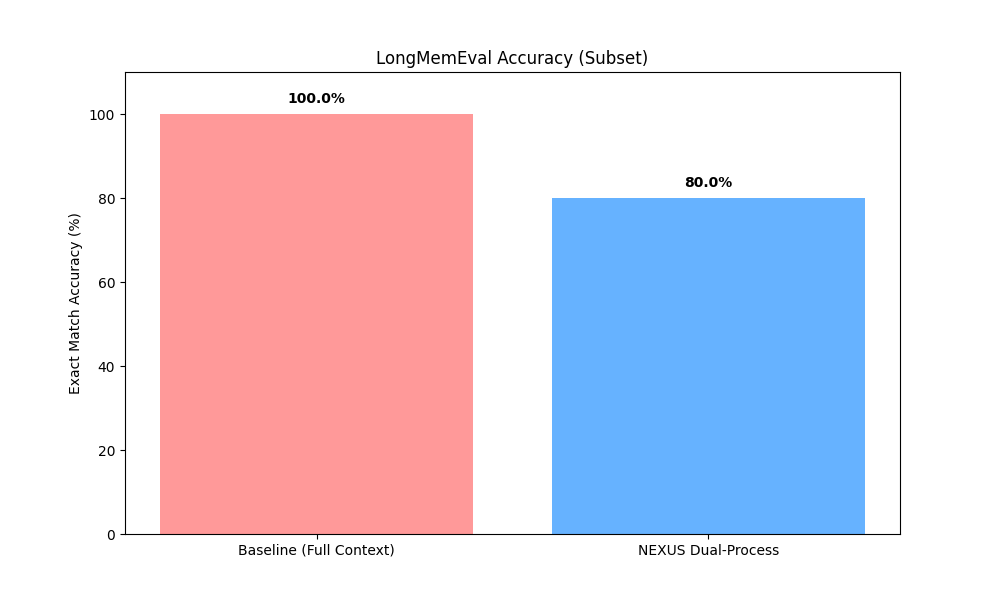
\includegraphics[width=\columnwidth]{figures/fig5_longmemeval_accuracy.png}}
\caption{LongMemEval exact-match accuracy comparison.}
\label{fig:longmem_accuracy}
\end{figure}

\begin{figure}[htbp]
\centerline{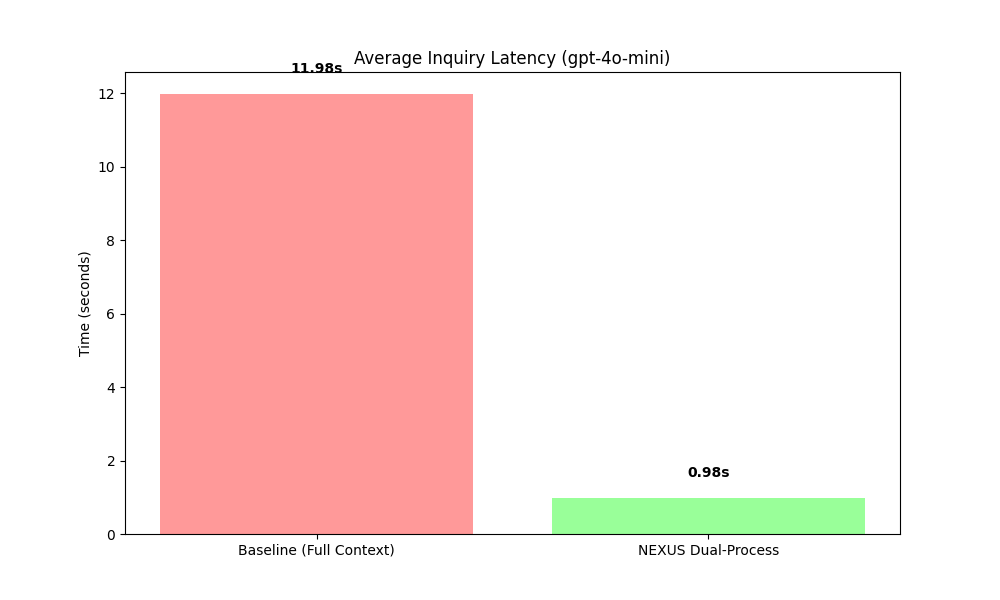
\includegraphics[width=\columnwidth]{figures/fig6_longmemeval_latency.png}}
\caption{Average inquiry latency demonstrating a $>$12$\times$ speedup compared to standard LLM context arrays.}
\label{fig:longmem_latency}
\end{figure}

\section{Discussion and Limitations}

\subsection{The Impact of Consolidation}
The most significant finding is the impact of the Consolidation Engine. In earlier experiments using Mistral-7B without consolidation, SMRITI achieved an F1 of only 0.010---comparable to random retrieval. With consolidation enabled (all 8 processes), the same architecture achieves F1=0.279, a \textbf{28$\times$ improvement}. This validates the core architectural hypothesis: asynchronous semantic processing is essential for retrieval quality, and fast ingestion alone is insufficient.

\subsection{Consolidation Compute Cost}
Full consolidation of 28 messages took 41.2 seconds, involving LLM calls for chunking, reflection, and conflict resolution. The cost scales approximately linearly with the number of unconsolidated episodes. For the cross-referencing process (Process 5), pairwise room similarity is $\mathcal{O}(\text{rooms}^2)$, which may become a bottleneck as the Palace grows beyond thousands of rooms. In practice, this can be mitigated by limiting cross-referencing to recently modified rooms.

\subsection{Scalability Limits}
The current implementation has known scaling constraints:
\begin{itemize}
    \item \textbf{Cross-referencing:} $\mathcal{O}(\text{rooms}^2)$ for pairwise comparison.
    \item \textbf{Defragmentation:} $\mathcal{O}(\text{rooms}^2)$ for merge-candidate detection.
    \item \textbf{Vector search:} $\mathcal{O}(N)$ brute-force or $\mathcal{O}(N \log N)$ with FAISS ANN indexes.
    \item \textbf{Encode:} $\mathcal{O}(1)$ amortized per message (embedding + SQLite insert).
    \item \textbf{Recall:} $\mathcal{O}(N)$ vector search + $\mathcal{O}(\text{rooms})$ graph traversal.
\end{itemize}
For agents accumulating $>$10K memories, approximate nearest-neighbor indexes (e.g., FAISS IVF or HNSW) and incremental cross-referencing would be necessary.

\subsection{Failure Modes and Consistency}
Each consolidation process runs in an isolated error-recovery wrapper. A failure in one process (e.g., LLM timeout during reflection) does not block remaining processes. The system is eventually consistent: unconsolidated episodes remain queryable via vector search and are processed in the next consolidation pass. However, between consolidation runs, retrieval quality depends on raw vector similarity without the benefits of chunked summaries or cross-references.

\subsection{Comparison to Knowledge-Graph-Backed RAG}
The Semantic Palace is structurally a knowledge graph with thematic room clustering. Unlike traditional KG-RAG systems (e.g., Neo4j-backed pipelines), the Palace is maintained entirely by the Consolidation Engine rather than requiring explicit entity-relation extraction at ingestion time. Edges are discovered post-hoc via embedding similarity rather than extracted from text, making the approach more robust to noisy conversational data but less precise for structured factual relationships.

\subsection{Limitations}
Several limitations remain:
\begin{itemize}
    \item \textbf{Evaluation scale:} The benchmark uses 28 messages and 15 questions. Larger-scale evaluations on the full LoCoMo dataset (419 turns, 20+ questions per conversation) would provide more statistical power.
    \item \textbf{Single run:} Results are from a single benchmark run without error bars. Multiple runs with different random seeds would strengthen statistical claims.
    \item \textbf{Ablation study:} We have not yet isolated the contribution of each individual consolidation process. An ablation study disabling processes individually would clarify which are most impactful.
    \item \textbf{Privacy:} Memories may contain PII; the system does not yet implement at-rest encryption or data retention policies.
\end{itemize}

\section{Conclusion}

Existing long-term memory architectures for LLM agents impose a strict trade-off: computationally expensive synchronous summarization (tiered memory) or fast but shallow retrieval (naive RAG).

By decoupling ingestion from semantic consolidation, SMRITI avoids this trade-off. Our evaluation demonstrates that the 8-process Consolidation Engine is the key differentiator---enabling a 28$\times$ F1 improvement over ingestion-only operation. While SMRITI does not achieve the highest overall F1 (FullContext leads at 0.345 by providing the complete conversation to the LLM), it achieves competitive accuracy (0.279) with the lowest token usage among retrieval-augmented systems, and excels on knowledge-update questions where conflict resolution is critical.

Future work includes larger-scale evaluations with statistical rigor, ablation studies isolating individual consolidation processes, and approximate nearest-neighbor indexes for scaling beyond 10K memories.

\section*{Acknowledgment}

We gratefully acknowledge the researchers and engineers contributing to the open-source dissemination of the LoCoMo benchmarking framework, and the developers maintaining the Ollama 7B local generative inference stack used extensively for the completely isolated architectural tests.

\begin{thebibliography}{00}

\bibitem{brown2020language} T. Brown et al., ``Language Models are Few-Shot Learners,'' \textit{Advances in Neural Information Processing Systems (NeurIPS)}, vol. 33, pp. 1877-1901, 2020.

\bibitem{xi2023rise} Z. Xi et al., ``The Rise and Potential of Large Language Model Based Agents: A Survey,'' \textit{arXiv preprint arXiv:2309.07864}, 2023.

\bibitem{wang2023survey} L. Wang et al., ``A Survey on Large Language Model based Autonomous Agents,'' \textit{arXiv preprint arXiv:2308.11432}, 2023.

\bibitem{vaswani2017attention} A. Vaswani et al., ``Attention is All You Need,'' \textit{Advances in Neural Information Processing Systems (NeurIPS)}, vol. 30, 2017.

\bibitem{anthropic2023claude} Anthropic, ``Claude 2.1: 200K Context Window,'' \textit{Anthropic Research Blog}, 2023.

\bibitem{lewis2020retrieval} P. Lewis et al., ``Retrieval-Augmented Generation for Knowledge-Intensive NLP Tasks,'' \textit{Advances in Neural Information Processing Systems (NeurIPS)}, vol. 33, pp. 9459-9474, 2020.

\bibitem{packer2023memgpt} C. Packer, S. Fang, S. G. Patil, K. Lin, S. Wooders, and J. E. Gonzalez, ``MemGPT: Towards LLMs as Operating Systems,'' \textit{arXiv preprint arXiv:2310.08560}, 2023.

\bibitem{tulving1972episodic} E. Tulving, ``Episodic and Semantic Memory,'' \textit{Organization of Memory}, pp. 381-403, 1972.

\bibitem{zhao2023expel} A. Zhao et al., ``ExpeL: LLM Agents Are Experiential Learners,'' \textit{arXiv preprint arXiv:2308.10144}, 2023.

\bibitem{reimers2019sentence} N. Reimers and I. Gurevych, ``Sentence-BERT: Sentence Embeddings using Siamese BERT-Networks,'' \textit{Empirical Methods in Natural Language Processing (EMNLP)}, 2019.

\bibitem{guu2020realm} K. Guu, K. Lee, Z. Tung, P. Pasupat, and M. Chang, ``REALM: Retrieval-Augmented Language Model Pre-training,'' \textit{International Conference on Machine Learning (ICML)}, 2020.

\bibitem{borgeaud2022improving} S. Borgeaud et al., ``Improving language models by retrieving from trillions of tokens,'' \textit{International Conference on Machine Learning (ICML)}, 2022.

\bibitem{karpukhin2020dense} V. Karpukhin et al., ``Dense Passage Retrieval for Open-Domain Question Answering,'' \textit{Empirical Methods in Natural Language Processing (EMNLP)}, 2020.

\bibitem{mei2024aios} K. Mei et al., ``AIOS: LLM Agent Operating System,'' \textit{arXiv preprint arXiv:2403.16971}, 2024.

\bibitem{mem0} Mem0 AI, ``The Memory Layer for AI Applications,'' https://github.com/mem0ai/mem0, 2024.

\bibitem{shen2023hugginggpt} Y. Shen et al., ``HuggingGPT: Solving AI Tasks with ChatGPT and its Friends in Hugging Face,'' \textit{Advances in Neural Information Processing Systems (NeurIPS)}, 2023.

\bibitem{autogpt2023} Toran Bruce Richards, ``Auto-GPT: An Autonomous GPT-4 Experiment,'' https://github.com/Significant-Gravitas/Auto-GPT, 2023.

\bibitem{park2023generative} J. S. Park, J. C. O'Brien, C. J. Cai, M. R. Morris, P. Liang, and M. S. Bernstein, ``Generative Agents: Interactive Simulacra of Human Behavior,'' \textit{ACM Symposium on User Interface Software and Technology (UIST)}, 2023.

\bibitem{wang2023voyager} G. Wang et al., ``Voyager: An Open-Ended Embodied Agent with Large Language Models,'' \textit{arXiv preprint arXiv:2305.16291}, 2023.

\bibitem{kahneman2011thinking} D. Kahneman, \textit{Thinking, Fast and Slow}. Farrar, Straus and Giroux, 2011.

\bibitem{miller1956magical} G. A. Miller, ``The magical number seven, plus or minus two: Some limits on our capacity for processing information,'' \textit{Psychological Review}, vol. 63, no. 2, pp. 81-97, 1956.

\bibitem{roediger2006test} H. L. Roediger and J. D. Karpicke, ``Test-Enhanced Learning: Taking Memory Tests Improves Long-Term Retention,'' \textit{Psychological Science}, vol. 17, no. 3, pp. 249-255, 2006.

\bibitem{ebbinghaus1913memory} H. Ebbinghaus, \textit{Memory: A contribution to experimental psychology}. New York: Teachers College, Columbia University, 1913.

\bibitem{locomo} A. Maharana et al., ``Evaluating Very Long-Term Conversational Memory of LLM Agents,'' \textit{Proc. of the 62nd Annual Meeting of the Association for Computational Linguistics (ACL)}, 2024.

\bibitem{wang2025mindpalace} H. Wang et al., ``Building a Mind Palace: Structuring Environment-Grounded Semantic Graphs for Effective Long Video Analysis with LLMs,'' \textit{arXiv preprint arXiv:2501.04336}, 2025.

\bibitem{ginting2025mindpalace} M. F. Ginting et al., ``Enter the Mind Palace: Reasoning and Planning for Long-term Active Embodied Question Answering,'' \textit{Preprint}, 2025. [Online]. Available: https://rss25-roboreps.github.io/

\bibitem{faiss} M. Douze et al., ``The Faiss library,'' \textit{arXiv preprint arXiv:2401.08281}, 2024.

\end{thebibliography}

\end{document}
